\documentclass[a4j]{jarticle}
\usepackage[dvipdfmx]{graphicx,color}
\usepackage{verbatim}
\usepackage{ascmac}
\usepackage{url}
\usepackage{listings,jlistings}
\usepackage{color}
%\setlength{\marginparwidth}{20mm}%% 傍注欄の横幅の設定

\input{/home/ryousuke/listings_temp.tex}

\title{情報科学プロジェクト実験レポート課題}
\author{S142063 佐藤涼亮}

\begin{document}
\maketitle
\centerline{\LARGE \underline{HTTP Cookie}}
\section{課題の内容}
{\large \underline{HTTP Cookieによるセッション管理}}
\subsection{要点}
\begin{enumerate}
\item あるHTTP要求に対してサーバは応答ヘッダにSet-Cookie:を設定する。
\item Webブラウザは設定されたその値をメモリまたはファイルに保存する。
\item Webブラウザは指定されたURLへのアクセスの際には、要求ヘッダにCookie:でその値を指定する。
\item サーバは要求ヘッダ内のCookie:の指定の有無で応答内容を変更する。\\(この値はCGIの環境変数HTTP\_COOKIEに設定される)
\end{enumerate}
\section{プログラムの説明}
ログイン画面と検索画面を作成し、それぞれのに対応した処理を行う。
ログイン画面には、ユーザー名とパスワードの入力欄を設け、
ログインに必要な情報の入力を求め、ログインを行う。
検索画面では、郵便番号入力欄を設け、
検索したい住所の情報の入力を求め、検索を行う。
それぞれ以下の4つの状況に応じた呼び出しと処理を行う。
\begin{itemize}
\item getメソッドでクッキー無しまたはDBに一致しないクッキー付きの場合\\
      ログイン画面を表示
\item getメソッドで、DBに一致するクッキー付きの場合\\
      検索画面を表示
\item postメソッドで、クッキー無しまたはDBに一致しないクッキー付きの場合\\
      ログイン画面を表示
\item postメソッドで、DBに一致するクッキー付きの場合\\
      pnumがなければ検索画面を表示\\pnumがあれば検索結果とともに検索画面を表示
\end{itemize}
\centerline{「DBに一致するクッキー」とは有効期限内のもののみとする}
有効期限は登録、更新した時刻から3分間とする。
\\
入力されたユーザー情報は、データベースに格納される。
ユーザー情報を格納するデータベースのテーブル、スキーマは以下の通りである。
\begin{screen}
\begin{verbatim}
sqlite> .table
account
sqlite> .schema
CREATE TABLE account (
user text not null,
pass text not null,
expire integer,
cookie text
);
\end{verbatim}
\end{screen}

\subsection{目的}
HTTP Cookieによるセッション管理

\subsection{方法}
HTTP Cookieによるセッション管理を用いて、
セッションにタイムアウト機能を設けたWebプログラムの実装

\subsection{結果}

\begin{center}
初期状態\\*

\includegraphics[width=\textwidth]{result/result1.png}\\*
ユーザー名にuser、パスワードにpasswordと入力しログインを行う

{\LARGE↓}

初めてのユーザー名の場合、パスワードと一緒に登録され\\*
検索画面が表示される\\*
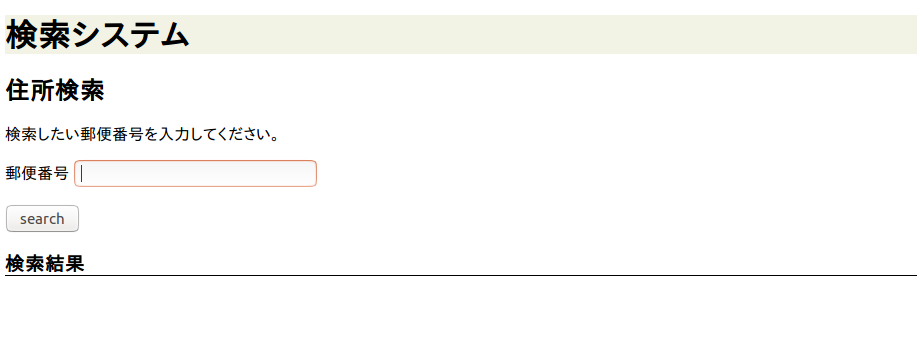
\includegraphics[width=\textwidth]{result/result2.png}\\*
検索したい郵便番号を入力し検索をする

{\LARGE↓}

検索画面に結果が追加され表示される\\*
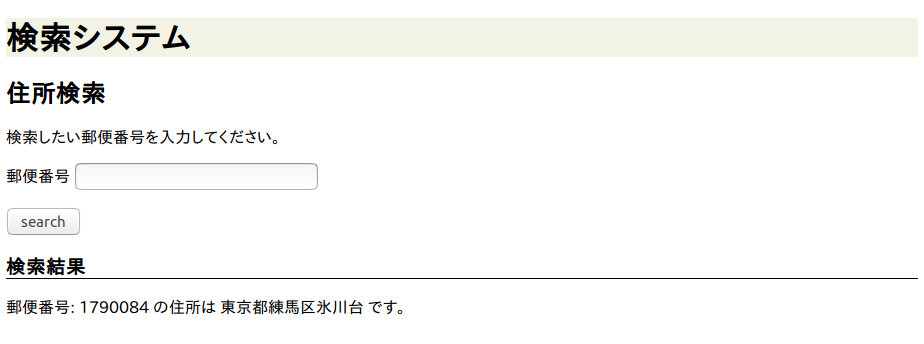
\includegraphics[width=\textwidth]{result/result3.png}\\*
有効期限内は検索が繰り返し行える。

{\LARGE↓}

セッションがタイムアウトすると\\*
ページがリロードされるときログイン画面に戻される\\*

\includegraphics[width=\textwidth]{result/result4.png}\\*
再度ログインするとCookieと有効期限が更新され検索画面が表示される
\\
入力に間違いがあると入力エラーとなる。\\*

\includegraphics[width=\textwidth]{result/result5.png}
\end{center}

\subsection{考察}
実行前のデータベースの状態は以下のとおりである。
\begin{screen}
\begin{verbatim}
sqlite> select * from account;
sqlite>
\end{verbatim}
\end{screen}\\

実行後、データベースは以下のとおりになる。
\begin{screen}
\begin{verbatim}
sqlite> select * from account;
user|password|1482230002|48727995
sqlite> 
\end{verbatim}
\end{screen}\\

再度ログイン後のデータベースは以下のとおりになる。
\begin{screen}
\begin{verbatim}
sqlite> select * from account;
user|password|1482231268|49741217
sqlite> 
\end{verbatim}
\end{screen}\\

これらより、データの格納・更新は成功し、
セッションのタイムアウトも行われたことから、期待通りの結果が得られた。

\section{感想}
今回、CGIプログラムにおいて、
HTTP Cookieにおけるセッション管理の機能を加えたプログラムを作成することができた。
この技術を用いて、成蹊ポータルのようなサイトの作成ををしてみたいと思った。
その上では、セキュリティの知識が必要となってくる。
なので、セキュリティについて今後学んでみたいと思う。
また、今回のプログラムに入力されたユーザー名やパスワードなどの使用可能かの検証を行えば、
より、いいサイトが作成できると思う。それにあたって、以前学んだAjaxの技術などを用いれるのではないかと考える。

\section{プログラム}
\lstinputlisting[caption=cookie.cpp]{cookie.cpp}

\end{document}
